% =============================================================================
% SECTION - FORCES CONSERVATIVES ET CONSERVATION DE L'ÉNERGIE MÉCANIQUE
% Chapitre 3 - Énergie et travail
% =============================================================================

\section{Forces conservatives et non-conservatives}
\label{sec:forces_conservatives}
% =============================================================================

Dans les sections précédentes, nous avons vu que certaines forces (comme la gravité et la force de rappel) permettent l'accumulation d'énergie potentielle, alors que d'autres (comme le frottement) ne le permettent pas. Cette distinction fondamentale mène à la classification des forces en deux catégories.

\subsection{Définition et propriétés}

\begin{definition}[title=Force conservative]
Une force est dite \textbf{conservative} si le travail qu'elle effectue sur un objet qui se déplace d'un point A à un point B est \textbf{indépendant du chemin} parcouru.

De manière équivalente, une force est conservative si le travail qu'elle effectue sur un objet qui parcourt un trajet fermé (retour au point de départ) est \textbf{nul}.
\end{definition}

\begin{definition}[title=Force non-conservative]
Une force est dite \textbf{non-conservative} si le travail qu'elle effectue \textbf{dépend du chemin} parcouru.

Pour une force non-conservative, le travail sur un trajet fermé est généralement \textbf{non nul}.
\end{definition}

\begin{remarque}[title=Classification des forces courantes]
\begin{center}
\renewcommand{\arraystretch}{1.3}
\begin{tabular}{|p{6cm}|p{6cm}|}
\hline
\rowcolor{bleuclair}
\textbf{Forces conservatives} & \textbf{Forces non-conservatives} \\
\hline
Force gravitationnelle ($\vect{F}_g$) & Force de frottement ($\vect{f}$) \\
Force de rappel d'un ressort ($\vect{F}_R$) & Force de résistance de l'air \\
Force électrostatique ($\vect{F}_E$) & Force motrice (poussée) \\
 & Force appliquée par une personne \\
 & Tension (dans la plupart des cas) \\
\hline
\end{tabular}
\end{center}
\end{remarque}

\subsection{Pourquoi cette distinction est-elle importante?}

\begin{center}
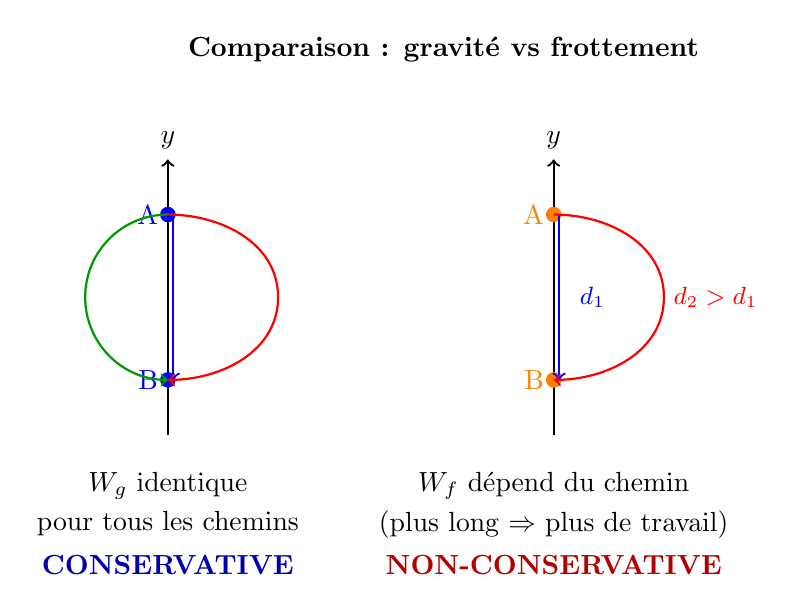
\begin{tikzpicture}[scale=0.7]
    % Titre
    \node[font=\bfseries] at (5,7) {Comparaison : gravité vs frottement};
    
    % Gauche : gravité (conservative)
    \draw[thick, ->] (0,0) -- (0,5) node[above] {$y$};
    \fill[blue] (0,4) circle (4pt) node[left] {A};
    \fill[blue] (0,1) circle (4pt) node[left] {B};
    
    % Chemins pour la gravité
    \draw[thick, blue, ->] (0.1,4) -- (0.1,1);
    \draw[thick, red, ->] (0,4) to[out=0, in=90] (2,2.5) to[out=-90, in=0] (0,1);
    \draw[thick, green!60!black, ->] (0,4) to[out=180, in=90] (-1.5,2.5) to[out=-90, in=180] (0,1);
    
    \node[below] at (0,-0.5) {$W_g$ identique};
    \node[below] at (0,-1.2) {pour tous les chemins};
    \node[below, font=\bfseries, blue!70!black] at (0,-2) {CONSERVATIVE};
    
    % Droite : frottement (non-conservative)
    \draw[thick, ->] (7,0) -- (7,5) node[above] {$y$};
    \fill[orange] (7,4) circle (4pt) node[left] {A};
    \fill[orange] (7,1) circle (4pt) node[left] {B};
    
    % Chemins pour le frottement
    \draw[thick, blue, ->] (7.1,4) -- (7.1,1);
    \node[right, blue] at (7.3,2.5) {\small $d_1$};
    \draw[thick, red, ->] (7,4) to[out=0, in=90] (9,2.5) to[out=-90, in=0] (7,1);
    \node[right, red] at (9,2.5) {\small $d_2 > d_1$};
    
    \node[below] at (7,-0.5) {$W_f$ dépend du chemin};
    \node[below] at (7,-1.2) {(plus long $\Rightarrow$ plus de travail)};
    \node[below, font=\bfseries, red!70!black] at (7,-2) {NON-CONSERVATIVE};
\end{tikzpicture}
\end{center}

\textbf{Conséquences fondamentales :}

\begin{itemize}
    \item Les forces \textbf{conservatives} permettent de définir une \textbf{énergie potentielle} associée. Le travail qu'elles effectuent peut être « récupéré ».
    \item Les forces \textbf{non-conservatives} ne permettent pas de définir une énergie potentielle. Le travail qu'elles effectuent est généralement « perdu » (transformé en chaleur, par exemple).
\end{itemize}

\begin{exemple}{Illustration avec un pendule}{}
Un pendule est un excellent exemple pour comprendre la différence :

\textbf{Pendule idéal (sans frottement) :}
\begin{itemize}
    \item Seule la gravité (force conservative) agit
    \item Le pendule oscille indéfiniment entre les mêmes hauteurs
    \item L'énergie se transforme continuellement entre $K$ et $U_g$, mais l'énergie totale reste constante
\end{itemize}

\textbf{Pendule réel (avec frottement) :}
\begin{itemize}
    \item Le frottement (force non-conservative) agit en plus de la gravité
    \item L'amplitude des oscillations diminue progressivement
    \item De l'énergie est « perdue » sous forme de chaleur à chaque oscillation
    \item Le pendule finit par s'arrêter
\end{itemize}

\begin{center}
\begin{tikzpicture}[scale=0.6]
    % Pendule idéal
    \draw[thick] (0,4) -- (0,5);
    \fill[pattern=north east lines] (-0.5,5) rectangle (0.5,5.3);
    
    % Trajectoire
    \draw[dashed, gray] (0,4) arc (270:240:3);
    \draw[dashed, gray] (0,4) arc (270:300:3);
    
    % Position gauche
    \draw[thick, blue] (0,5) -- (-2.6,2.5);
    \fill[blue] (-2.6,2.5) circle (6pt);
    
    % Position droite (fantôme)
    \draw[thick, blue, dashed] (0,5) -- (2.6,2.5);
    \fill[blue, opacity=0.3] (2.6,2.5) circle (6pt);
    
    % Position basse
    \draw[thick, gray, dashed] (0,5) -- (0,2);
    \fill[gray, opacity=0.3] (0,2) circle (6pt);
    
    % Flèches
    \draw[very thick, ->, green!60!black] (-2.6,2.5) to[out=-30, in=180] (0,1.5) to[out=0, in=-150] (2.6,2.5);
    
    \node[below] at (0,0) {\textbf{Pendule idéal}};
    \node[below] at (0,-0.7) {Même hauteur atteinte};
    
    % Pendule réel
    \draw[thick] (8,4) -- (8,5);
    \fill[pattern=north east lines] (7.5,5) rectangle (8.5,5.3);
    
    % Trajectoire décroissante
    \draw[thick, red] (8,5) -- (5.4,2.5);
    \fill[red] (5.4,2.5) circle (6pt);
    
    \draw[thick, red, dashed] (8,5) -- (9.8,3.2);
    \fill[red, opacity=0.5] (9.8,3.2) circle (6pt);
    
    % Flèches décroissantes
    \draw[very thick, ->, orange] (5.4,2.5) to[out=-30, in=180] (8,1.8) to[out=0, in=-150] (9.8,3.2);
    
    \node[below] at (8,0) {\textbf{Pendule réel}};
    \node[below] at (8,-0.7) {Amplitude décroissante};
\end{tikzpicture}
\end{center}
\end{exemple}

% =============================================================================
\section{Conservation de l'énergie mécanique}
\label{sec:conservation_energie}
% =============================================================================

\subsection{Énergie mécanique}

\begin{definition}[title=Énergie mécanique]
L'\textbf{énergie mécanique} $E$ d'un système est la somme de son énergie cinétique $K$ et de son énergie potentielle $U$ :

\begin{equationimportante}
\begin{equation}
E = K + U
\label{eq:energie_mecanique}
\end{equation}
\end{equationimportante}

où :
\begin{itemize}
    \item $K = \frac{1}{2}mv^2$ est l'énergie cinétique
    \item $U = U_g + U_e$ est l'énergie potentielle totale (gravitationnelle + élastique, si applicable)
\end{itemize}
\end{definition}

\subsection{Principe de conservation}

Lorsqu'un système n'est soumis qu'à des forces conservatives, quelque chose de remarquable se produit : l'énergie mécanique totale reste constante.

\begin{definition}[title=Conservation de l'énergie mécanique]
En l'absence de forces non-conservatives, l'énergie mécanique d'un système se conserve :

\begin{equationimportante}
\begin{equation}
E_i = E_f \quad \Leftrightarrow \quad K_i + U_i = K_f + U_f
\label{eq:conservation_energie}
\end{equation}
\end{equationimportante}

De manière équivalente : $\Delta E = 0$ ou $\Delta K + \Delta U = 0$
\end{definition}

\begin{remarque}[title=Démonstration]
Par le théorème de l'énergie cinétique : $W_{\text{total}} = \Delta K$

Si seules des forces conservatives agissent, alors : $W_{\text{total}} = W_c = -\Delta U$

Donc : $\Delta K = -\Delta U$, ce qui donne $\Delta K + \Delta U = 0$, soit $E_f = E_i$.
\end{remarque}

\begin{attention}[title=Quand utiliser la conservation de l'énergie?]
Le principe de conservation de l'énergie mécanique s'applique \textbf{uniquement} lorsque :
\begin{itemize}
    \item Aucune force non-conservative n'effectue de travail sur le système
    \item Ou le travail des forces non-conservatives est négligeable
\end{itemize}

En pratique, cela signifie : \textbf{pas de frottement}, \textbf{pas de résistance de l'air}, \textbf{pas de force motrice externe}.
\end{attention}

% =============================================================================
\subsection{L'algorithme de résolution par méthode énergétique}
\label{subsec:algorithme-energie}
% =============================================================================

Résoudre un problème par la méthode énergétique est souvent plus simple qu'utiliser les lois de Newton, car l'énergie est une grandeur \textbf{scalaire} --- pas besoin de décomposer en composantes $x$ et $y$! En revanche, cette méthode exige un bilan énergétique rigoureux.

\begin{definition}[title=Algorithme de résolution par méthode énergétique (4 étapes)]

\textbf{Étape 1 --- SCHÉMA et ÉTATS}
\begin{enumerate}[label=\alph*)]
    \item Dessiner un schéma de la situation physique
    \item Identifier clairement l'\textbf{état initial} (i) et l'\textbf{état final} (f)
    \item Choisir un \textbf{niveau de référence} pour l'énergie potentielle ($y = 0$)
    \item Indiquer les grandeurs connues et inconnues à chaque état ($v_i$, $v_f$, $y_i$, $y_f$, $x_i$, $x_f$)
\end{enumerate}

\vspace{0.5em}
\textbf{Étape 2 --- BILAN ÉNERGÉTIQUE}
\begin{enumerate}[label=\alph*)]
    \item Lister les formes d'énergie \textbf{présentes} à l'état initial : $K_i$, $U_{gi}$, $U_{ei}$
    \item Lister les formes d'énergie \textbf{présentes} à l'état final : $K_f$, $U_{gf}$, $U_{ef}$
    \item Identifier les forces non-conservatives qui effectuent un travail ($W_{nc}$) : frottement, force motrice, résistance de l'eau...
    \item Si $W_{nc} = 0$ : conservation de l'énergie mécanique ($E_i = E_f$)
    \item Si $W_{nc} \neq 0$ : bilan complet ($E_i + W_{nc} = E_f$)
\end{enumerate}

\vspace{0.5em}
\textbf{Étape 3 --- ÉQUATION D'ÉNERGIE}
\begin{enumerate}[label=\alph*)]
    \item Écrire l'équation de conservation complète :
    \[ K_i + U_{gi} + U_{ei} + W_{nc} = K_f + U_{gf} + U_{ef} \]
    \item Éliminer les termes nuls (objet au repos? au niveau de référence? pas de ressort?)
    \item Remplacer chaque terme par son expression algébrique
\end{enumerate}

\vspace{0.5em}
\textbf{Étape 4 --- ALGÈBRE}
\begin{enumerate}[label=\alph*)]
    \item Isoler l'inconnue \textbf{algébriquement} (avec des symboles)
    \item Substituer les valeurs numériques \textit{à la fin}
    \item Vérifier : unités correctes? Ordre de grandeur raisonnable? Signe cohérent?
\end{enumerate}
\end{definition}

\begin{remarque}[title=Quand choisir la méthode énergétique plutôt que les lois de Newton?]
\begin{itemize}
    \item \textbf{Méthode énergétique} : quand on s'intéresse à la \textbf{vitesse} à un point donné, sans avoir besoin de connaître l'accélération ou les forces individuelles. Idéale pour les trajectoires courbes ou les situations avec plusieurs forces.
    \item \textbf{Lois de Newton} : quand on cherche une \textbf{force} spécifique (tension, normale, etc.) ou l'\textbf{accélération} du système.
\end{itemize}
Les deux méthodes donnent toujours le même résultat --- le choix est une question d'efficacité.
\end{remarque}

\subsection{Applications de la conservation de l'énergie}

\begin{exemple}{Chute libre d'un conteneur}{}
Un conteneur de masse $m = \SI{8000}{kg}$ tombe accidentellement d'une hauteur de $h = \SI{10}{m}$. En négligeant la résistance de l'air, calculez sa vitesse juste avant l'impact.

\textbf{Système :} Le conteneur\\
\textbf{Forces :} Gravité (conservative)\\
\textbf{Conclusion :} L'énergie mécanique se conserve.

\begin{center}
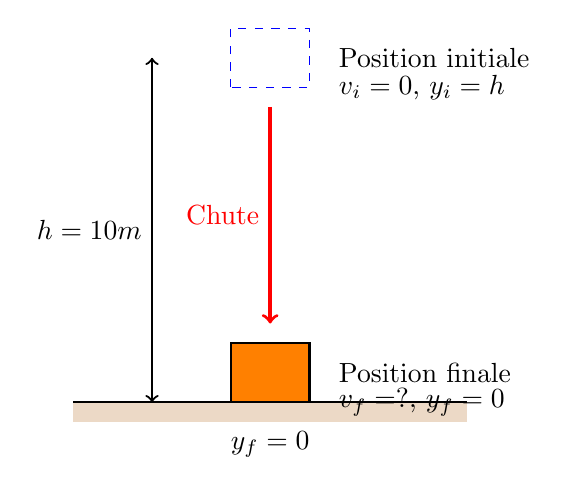
\begin{tikzpicture}[scale=0.5]
    % Sol
    \fill[brown!30] (-2,-0.5) rectangle (8,0);
    \draw[thick] (-2,0) -- (8,0);
    \node[below] at (3,-0.5) {$y_f = 0$};
    
    % Position initiale
    \draw[dashed, blue] (2,8) rectangle (4,9.5);
    \node[right] at (4.5,8.75) {Position initiale};
    \node[right] at (4.5,8) {$v_i = 0$, $y_i = h$};
    
    % Position finale
    \fill[orange] (2,0) rectangle (4,1.5);
    \draw[thick] (2,0) rectangle (4,1.5);
    \node[right] at (4.5,0.75) {Position finale};
    \node[right] at (4.5,0) {$v_f = ?$, $y_f = 0$};
    
    % Flèche de chute
    \draw[very thick, ->, red] (3,7.5) -- (3,2) node[midway, left] {Chute};
    
    % Hauteur
    \draw[<->, thick] (0,0) -- (0,8.75) node[midway, left] {$h = \SI{10}{m}$};
\end{tikzpicture}
\end{center}

\textbf{Application de la conservation de l'énergie :}
\[ E_i = E_f \]
\[ K_i + U_{g,i} = K_f + U_{g,f} \]
\[ \frac{1}{2}mv_i^2 + mgy_i = \frac{1}{2}mv_f^2 + mgy_f \]

Avec $v_i = 0$, $y_i = h$ et $y_f = 0$ :
\[ 0 + mgh = \frac{1}{2}mv_f^2 + 0 \]
\[ mgh = \frac{1}{2}mv_f^2 \]

On peut simplifier par $m$ :
\[ gh = \frac{1}{2}v_f^2 \]
\[ v_f = \sqrt{2gh} = \sqrt{2 \times 9,8 \times 10} = \sqrt{196} = \SI{14}{m/s} \]

\begin{remarque}
Notez que la masse s'annule! La vitesse de chute libre ne dépend pas de la masse, seulement de la hauteur. C'est le même résultat que Galilée a découvert il y a plus de 400 ans.
\end{remarque}
\end{exemple}

\begin{exemple}{Navire sur une vague (modèle simplifié)}{}
Un petit bateau de masse $m = \SI{500}{kg}$ descend une vague. Au sommet de la vague (point A), le bateau est momentanément immobile à une hauteur de \SI{3}{m} au-dessus du creux. Quelle est sa vitesse au point le plus bas (point B)?

Hypothèses : On néglige la résistance de l'eau et on traite le bateau comme une particule.

\begin{center}
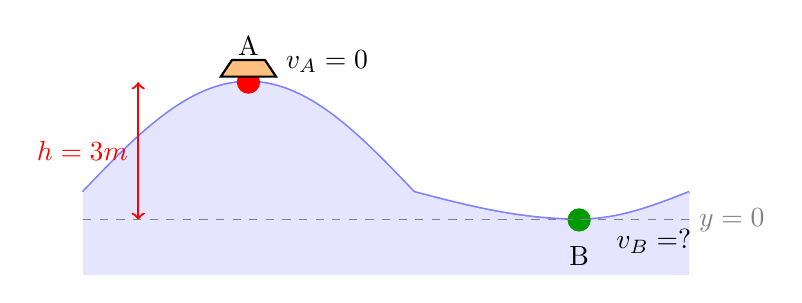
\begin{tikzpicture}[scale=0.7]
    % Vague
    \draw[very thick, blue!50] (-1,0) sin (2,2) cos (5,0) sin (8,-0.5) cos (10,0);
    \fill[blue!10] (-1,0) sin (2,2) cos (5,0) sin (8,-0.5) cos (10,0) -- (10,-1.5) -- (-1,-1.5) -- cycle;
    
    % Point A (sommet)
    \fill[red] (2,2) circle (6pt);
    \node[above] at (2,2.3) {A};
    \node[above right] at (2.5,2) {$v_A = 0$};
    
    % Point B (creux)
    \fill[green!60!black] (8,-0.5) circle (6pt);
    \node[below] at (8,-0.8) {B};
    \node[below right] at (8.5,-0.5) {$v_B = ?$};
    
    % Hauteur
    \draw[<->, thick, red] (0,2) -- (0,-0.5) node[midway, left] {$h = \SI{3}{m}$};
    
    % Niveau de référence
    \draw[dashed, gray] (-1,-0.5) -- (10,-0.5);
    \node[right, gray] at (10,-0.5) {$y = 0$};
    
    % Bateau simplifié au point A
    \draw[thick, fill=orange!50] (1.5,2.1) -- (2.5,2.1) -- (2.3,2.4) -- (1.7,2.4) -- cycle;
\end{tikzpicture}
\end{center}

\textbf{Conservation de l'énergie :}
\[ E_A = E_B \]
\[ K_A + U_{g,A} = K_B + U_{g,B} \]

En prenant le creux (point B) comme niveau de référence ($y_B = 0$) :
\[ 0 + mgh = \frac{1}{2}mv_B^2 + 0 \]
\[ v_B = \sqrt{2gh} = \sqrt{2 \times 9,8 \times 3} = \SI{7,7}{m/s} \approx \SI{15}{\knots} \]

Le bateau atteint une vitesse de près de 15 nœuds au bas de la vague!
\end{exemple}

\begin{pratiqueautonome}
Une bille de masse $m = \SI{0,5}{kg}$ est lâchée du repos au sommet d'une glissière sans frottement de hauteur $h = \SI{2}{m}$.

\begin{enumerate}[label=\alph*)]
    \item Quelle est l'énergie mécanique totale de la bille? (Prenez le bas de la glissière comme référence.)
    \item Quelle est sa vitesse au bas de la glissière?
    \item Si la bille remonte ensuite une autre pente, à quelle hauteur maximale pourra-t-elle s'élever?
\end{enumerate}

\espaceresolution[6cm]
\reponsepratique{a) $E = mgh = \SI{9,8}{J}$ \quad b) $v = \sqrt{2gh} = \SI{6,26}{m/s}$ \quad c) $h_{\max} = \SI{2}{m}$ (même hauteur qu'au départ)}
\end{pratiqueautonome}

\begin{exemple}{Pendule simple}{}
Un pendule de longueur $L = \SI{1,5}{m}$ est écarté de $\theta = 30\si{\degree}$ de la verticale, puis lâché. Quelle est sa vitesse au point le plus bas de sa trajectoire?

\begin{center}
\begin{tikzpicture}[scale=1]
    % Point de suspension
    \fill[pattern=north east lines] (-0.3,3) rectangle (0.3,3.3);
    \draw[thick] (-0.3,3) -- (0.3,3);
    
    % Position initiale (écartée)
    \draw[thick, gray] (0,3) -- (-1.3,1.5);
    \fill[blue] (-1.3,1.5) circle (6pt);
    \node[left] at (-1.5,1.5) {A};
    
    % Position finale (verticale)
    \draw[thick, dashed, gray] (0,3) -- (0,1.5);
    \fill[green!60!black] (0,1.5) circle (6pt);
    \node[right] at (0.2,1.5) {B};
    
    % Arc de trajectoire
    \draw[dashed, blue!50] (-1.3,1.5) arc (210:270:1.5);
    
    % Angle
    \draw[thick] (0,3) -- (0,2.3);
    \draw[->] (0,2.5) arc (270:210:0.5) node[midway, below left] {$\theta$};
    
    % Longueur
    \node[above left] at (-0.7,2.3) {$L$};
    
    % Hauteur h
    \draw[<->, thick, red] (0.5,1.5) -- (0.5,2.2) node[midway, right] {$h$};
    \draw[dashed, gray] (-1.3,1.5) -- (0.5,1.5);
    \draw[dashed, gray] (-1.3,2.2) -- (0.5,2.2);
    
    % Niveau B
    \node[right] at (1,1.5) {$y = 0$};
\end{tikzpicture}
\end{center}

\textbf{Calcul de la hauteur initiale :}

Par géométrie, la hauteur du point A au-dessus du point B est :
\[ h = L - L\cos\theta = L(1 - \cos\theta) \]
\[ h = 1,5 \times (1 - \cos 30\si{\degree}) = 1,5 \times (1 - 0,866) = 1,5 \times 0,134 = \SI{0,201}{m} \]

\textbf{Conservation de l'énergie :}
\[ E_A = E_B \]
\[ mgh = \frac{1}{2}mv_B^2 \]
\[ v_B = \sqrt{2gh} = \sqrt{2 \times 9,8 \times 0,201} = \SI{1,98}{m/s} \]
\end{exemple}

\begin{pratiqueautonome}
Un pendule de longueur $L = \SI{2}{m}$ passe par sa position d'équilibre (point le plus bas) avec une vitesse de $v = \SI{3}{m/s}$.

\begin{enumerate}[label=\alph*)]
    \item Quelle hauteur maximale atteindra-t-il de chaque côté?
    \item Quel angle maximal fera-t-il avec la verticale?
\end{enumerate}

\espaceresolution[5cm]
\reponsepratique{a) $h = v^2/(2g) = \SI{0,459}{m}$ \quad b) $\theta = \arccos(1 - h/L) = \arccos(0,770) \approx 39,6\si{\degree}$}
\end{pratiqueautonome}
\subsection{Conservation de l'énergie avec forces non-conservatives}

Dans la réalité, le frottement et d'autres forces non-conservatives sont presque toujours présents. L'énergie mécanique n'est alors plus conservée, mais l'énergie \textbf{totale} (incluant l'énergie thermique) l'est toujours.

\begin{definition}[title=Bilan énergétique avec forces non-conservatives]
Lorsque des forces non-conservatives agissent sur un système, la variation de l'énergie mécanique est égale au travail effectué par ces forces :

\begin{equationimportante}
\begin{equation}
W_{nc} = \Delta E = E_f - E_i = (K_f + U_f) - (K_i + U_i)
\label{eq:energie_non_conservative}
\end{equation}
\end{equationimportante}

De manière équivalente :
\begin{equation}
K_i + U_i + W_{nc} = K_f + U_f
\label{eq:bilan_energetique}
\end{equation}
\end{definition}

\begin{remarque}[title=Interprétation du travail des forces non-conservatives]
\begin{itemize}
    \item Si $W_{nc} > 0$ (force motrice, poussée) : l'énergie mécanique \textbf{augmente}
    \item Si $W_{nc} < 0$ (frottement, résistance) : l'énergie mécanique \textbf{diminue}
\end{itemize}

Le frottement effectue toujours un travail négatif car il s'oppose au mouvement. L'énergie « perdue » est en fait transformée en chaleur.
\end{remarque}

\begin{attention}[title=L'énergie totale se conserve toujours!]
Le principe fondamental de conservation de l'énergie stipule que l'énergie ne peut être ni créée ni détruite, seulement transformée. Lorsque le frottement fait « perdre » de l'énergie mécanique, cette énergie est en fait convertie en \textbf{énergie thermique} (chaleur).

\[ E_{\text{mécanique}} + E_{\text{thermique}} = \text{constante} \]

C'est pourquoi les freins d'un véhicule chauffent lors d'un freinage prolongé!
\end{attention}

\begin{exemple}{Freinage d'un navire avec frottement de l'eau}{}
Un navire de masse $m = \SI{15000}{tonnes}$ navigue à $v_i = \SI{6}{m/s}$. Les moteurs sont coupés et le navire ralentit uniquement sous l'effet de la résistance de l'eau jusqu'à $v_f = \SI{2}{m/s}$ après avoir parcouru $d = \SI{800}{m}$. Quelle est la force moyenne de résistance de l'eau?

\textbf{Bilan énergétique :}

Le navire se déplace horizontalement, donc $\Delta U_g = 0$.

\[ W_{nc} = \Delta K = K_f - K_i \]
\[ W_{nc} = \frac{1}{2}mv_f^2 - \frac{1}{2}mv_i^2 \]
\[ W_{nc} = \frac{1}{2} \times \SI{15e6}{kg} \times [(\SI{2}{m/s})^2 - (\SI{6}{m/s})^2] \]
\[ W_{nc} = \frac{1}{2} \times \SI{15e6}{} \times (4 - 36) = \frac{1}{2} \times \SI{15e6}{} \times (-32) \]
\[ W_{nc} = -\SI{240e6}{J} = -\SI{240}{MJ} \]

\textbf{Calcul de la force de résistance :}

Le travail de la résistance est $W_{nc} = -F_r \times d$ (négatif car opposé au mouvement) :
\[ -F_r \times 800 = -\SI{240e6}{J} \]
\[ F_r = \frac{\SI{240e6}{J}}{\SI{800}{m}} = \SI{300000}{N} = \SI{300}{kN} \]

La force moyenne de résistance de l'eau est d'environ \textbf{\SI{300}{kN}}.
\end{exemple}

\begin{exemple}{Descente d'une rampe avec frottement}{}
Une caisse de $m = \SI{50}{kg}$ glisse sur une rampe inclinée à $30\si{\degree}$, parcourant une distance de $d = \SI{4}{m}$ le long de la rampe. Le coefficient de frottement cinétique est $\mu_c = 0,25$. Si la caisse part du repos, quelle est sa vitesse au bas de la rampe?

\begin{center}
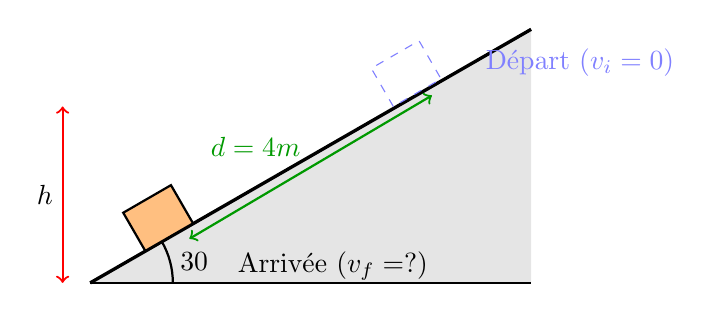
\begin{tikzpicture}[scale=0.7]
    % Plan incliné
    \fill[gray!20] (0,0) -- (8,0) -- (8,4.6) -- cycle;
    \draw[very thick] (0,0) -- (8,4.6);
    \draw[thick] (0,0) -- (8,0);
    
    % Angle
    \draw[thick] (1.5,0) arc (0:30:1.5) node[midway, right] {$30\si{\degree}$};
    
    % Caisse position initiale
    \begin{scope}[shift={(5.5,3.2)}, rotate=30]
        \draw[dashed, blue!50] (0,0) rectangle (1,0.8);
    \end{scope}
    \node[blue!50, right] at (7,4) {Départ ($v_i = 0$)};
    
    % Caisse position finale
    \begin{scope}[shift={(1,0.58)}, rotate=30]
        \fill[orange!50] (0,0) rectangle (1,0.8);
        \draw[thick] (0,0) rectangle (1,0.8);
    \end{scope}
    \node[right] at (2.5,0.3) {Arrivée ($v_f = ?$)};
    
    % Hauteur
    \draw[<->, thick, red] (-0.5,0) -- (-0.5,3.2);
    \node[left] at (-0.5,1.6) {$h$};
    
    % Distance
    \draw[<->, thick, green!60!black] (1.8,0.8) -- (6.2,3.4) node[midway, above left] {$d = \SI{4}{m}$};
\end{tikzpicture}
\end{center}

\textbf{Calcul de la hauteur :}
\[ h = d\sin(30\si{\degree}) = 4 \times 0,5 = \SI{2}{m} \]

\textbf{Calcul de la force de frottement :}
\[ N = mg\cos(30\si{\degree}) = 50 \times 9,8 \times 0,866 = \SI{424}{N} \]
\[ f = \mu_c N = 0,25 \times 424 = \SI{106}{N} \]

\textbf{Travail du frottement :} (opposé au déplacement)
\[ W_f = -fd = -106 \times 4 = -\SI{424}{J} \]

\textbf{Bilan énergétique :}
\[ K_i + U_i + W_{nc} = K_f + U_f \]
\[ 0 + mgh + W_f = \frac{1}{2}mv_f^2 + 0 \]
\[ 50 \times 9,8 \times 2 + (-424) = \frac{1}{2} \times 50 \times v_f^2 \]
\[ 980 - 424 = 25 v_f^2 \]
\[ v_f^2 = \frac{556}{25} = 22,24 \]
\[ v_f = \sqrt{22,24} = \SI{4,7}{m/s} \]

\begin{remarque}
Sans frottement, la vitesse aurait été $v = \sqrt{2gh} = \sqrt{2 \times 9,8 \times 2} = \SI{6,3}{m/s}$. Le frottement a réduit la vitesse finale de près de 25\%.
\end{remarque}
\end{exemple}

\begin{pratiqueautonome}
Un traîneau de $m = \SI{80}{kg}$ est tiré sur une surface horizontale enneigée par une force de $F = \SI{200}{N}$ parallèle au sol. Le coefficient de frottement cinétique est $\mu_c = 0,15$. Le traîneau part du repos.

\begin{enumerate}[label=\alph*)]
    \item Calculez le travail effectué par la force de traction sur une distance de \SI{10}{m}.
    \item Calculez le travail effectué par le frottement sur cette distance.
    \item En utilisant le bilan énergétique, déterminez la vitesse du traîneau après \SI{10}{m}.
\end{enumerate}

\espaceresolution[7cm]
\reponsepratique{a) $W_F = 200 \times 10 = \SI{2000}{J}$ \quad b) $W_f = -\mu_c mg \times d = -0,15 \times 80 \times 9,8 \times 10 = -\SI{1176}{J}$ \quad c) $\Delta K = W_F + W_f = 824$~J, donc $v = \sqrt{2 \times 824/80} = \SI{4,5}{m/s}$}
\end{pratiqueautonome}

% =============================================================================
